\documentclass[a4paper]{article}

\def\npart {II}
\def\nterm {Michaelmas}
\def\nyear {2015}
\def\nlecturer {C. Birkar}
\def\ncourse {Galois Theory}
\def\nlectures {TTS.12}
\def\nnotready {}

% Imports
\ifx \nextra \undefined
  \usepackage[pdftex,
    hidelinks,
    pdfauthor={Dexter Chua},
    pdfsubject={Cambridge Maths Notes: Part \npart\ - \ncourse},
    pdftitle={Part \npart\ - \ncourse},
  pdfkeywords={Cambridge Mathematics Maths Math \npart\ \nterm\ \nyear\ \ncourse}]{hyperref}
  \title{Part \npart\ - \ncourse}
\else
  \usepackage[pdftex,
    hidelinks,
    pdfauthor={Dexter Chua},
    pdfsubject={Cambridge Maths Notes: Part \npart\ - \ncourse\ (\nextra)},
    pdftitle={Part \npart\ - \ncourse\ (\nextra)},
  pdfkeywords={Cambridge Mathematics Maths Math \npart\ \nterm\ \nyear\ \ncourse\ \nextra}]{hyperref}

  \title{Part \npart\ - \ncourse \\ {\Large \nextra}}
\fi

\author{Lectured by \nlecturer \\\small Notes taken by Dexter Chua}
\date{\nterm\ \nyear}

\usepackage{alltt}
\usepackage{amsfonts}
\usepackage{amsmath}
\usepackage{amssymb}
\usepackage{amsthm}
\usepackage{booktabs}
\usepackage{caption}
\usepackage{enumitem}
\usepackage{fancyhdr}
\usepackage{graphicx}
\usepackage{mathtools}
\usepackage{microtype}
\usepackage{multirow}
\usepackage{pdflscape}
\usepackage{pgfplots}
\usepackage{siunitx}
\usepackage{tabularx}
\usepackage{tikz}
\usepackage{tkz-euclide}
\usepackage[normalem]{ulem}
\usepackage[all]{xy}

\pgfplotsset{compat=1.12}

\pagestyle{fancyplain}
\lhead{\emph{\nouppercase{\leftmark}}}
\ifx \nextra \undefined
  \rhead{
    \ifnum\thepage=1
    \else
      \npart\ \ncourse
    \fi}
\else
  \rhead{
    \ifnum\thepage=1
    \else
      \npart\ \ncourse\ (\nextra)
    \fi}
\fi
\usetikzlibrary{arrows}
\usetikzlibrary{decorations.markings}
\usetikzlibrary{decorations.pathmorphing}
\usetikzlibrary{positioning}
\usetikzlibrary{fadings}
\usetikzlibrary{intersections}
\usetikzlibrary{cd}

\newcommand*{\Cdot}{\raisebox{-0.25ex}{\scalebox{1.5}{$\cdot$}}}
\newcommand {\pd}[2][ ]{
  \ifx #1 { }
    \frac{\partial}{\partial #2}
  \else
    \frac{\partial^{#1}}{\partial #2^{#1}}
  \fi
}

% Theorems
\theoremstyle{definition}
\newtheorem*{aim}{Aim}
\newtheorem*{axiom}{Axiom}
\newtheorem*{claim}{Claim}
\newtheorem*{cor}{Corollary}
\newtheorem*{defi}{Definition}
\newtheorem*{eg}{Example}
\newtheorem*{fact}{Fact}
\newtheorem*{law}{Law}
\newtheorem*{lemma}{Lemma}
\newtheorem*{notation}{Notation}
\newtheorem*{prop}{Proposition}
\newtheorem*{thm}{Theorem}

\renewcommand{\labelitemi}{--}
\renewcommand{\labelitemii}{$\circ$}
\renewcommand{\labelenumi}{(\roman{*})}

\let\stdsection\section
\renewcommand\section{\newpage\stdsection}

% Strike through
\def\st{\bgroup \ULdepth=-.55ex \ULset}

% Maths symbols
\newcommand{\bra}{\langle}
\newcommand{\ket}{\rangle}

\newcommand{\N}{\mathbb{N}}
\newcommand{\Z}{\mathbb{Z}}
\newcommand{\Q}{\mathbb{Q}}
\renewcommand{\H}{\mathbb{H}}
\newcommand{\R}{\mathbb{R}}
\newcommand{\C}{\mathbb{C}}
\newcommand{\Prob}{\mathbb{P}}
\renewcommand{\P}{\mathbb{P}}
\newcommand{\E}{\mathbb{E}}
\newcommand{\F}{\mathbb{F}}
\newcommand{\cU}{\mathcal{U}}
\newcommand{\RP}{\mathbb{RP}}
\newcommand{\CP}{\mathbb{CP}}

\newcommand{\ph}{\,\cdot\,}

\DeclareMathOperator{\sech}{sech}
\DeclareMathOperator{\cosech}{cosech}
\DeclareMathOperator{\cosec}{cosec}

\DeclareMathOperator{\covol}{covol}
\DeclareMathOperator{\vol}{vol}

\let\Im\relax
\let\Re\relax
\DeclareMathOperator{\Im}{Im}
\DeclareMathOperator{\Re}{Re}
\DeclareMathOperator{\im}{im}
\DeclareMathOperator{\image}{image}
\DeclareMathOperator{\Ann}{Ann}

\DeclareMathOperator*{\res}{res}
\DeclareMathOperator{\Res}{Res}
\DeclareMathOperator{\Ind}{Ind}

\DeclareMathOperator{\tr}{tr}
\DeclareMathOperator{\diag}{diag}
\DeclareMathOperator{\rank}{rank}
\DeclareMathOperator{\card}{card}
\DeclareMathOperator{\spn}{span}
\DeclareMathOperator{\adj}{adj}

\DeclareMathOperator{\erf}{erf}
\DeclareMathOperator{\erfc}{erfc}

\DeclareMathOperator{\ord}{ord}
\DeclareMathOperator{\Sym}{Sym}

\DeclareMathOperator{\sgn}{sgn}
\DeclareMathOperator{\orb}{orb}
\DeclareMathOperator{\stab}{stab}
\DeclareMathOperator{\ccl}{ccl}

\DeclareMathOperator{\lcm}{lcm}
\DeclareMathOperator{\hcf}{hcf}

\DeclareMathOperator{\Int}{Int}
\DeclareMathOperator{\id}{id}

\DeclareMathOperator{\betaD}{beta}
\DeclareMathOperator{\gammaD}{gamma}
\DeclareMathOperator{\Poisson}{Poisson}
\DeclareMathOperator{\binomial}{binomial}
\DeclareMathOperator{\multinomial}{multinomial}
\DeclareMathOperator{\Bernoulli}{Bernoulli}
\DeclareMathOperator{\like}{like}

\DeclareMathOperator{\var}{var}
\DeclareMathOperator{\cov}{cov}
\DeclareMathOperator{\bias}{bias}
\DeclareMathOperator{\mse}{mse}
\DeclareMathOperator{\corr}{corr}

\DeclareMathOperator{\otp}{otp}
\DeclareMathOperator{\dom}{dom}

\DeclareMathOperator{\Root}{Root}
\DeclareMathOperator{\supp}{supp}
\DeclareMathOperator{\rel}{rel}
\DeclareMathOperator{\Hom}{Hom}
\DeclareMathOperator{\Aut}{Aut}
\DeclareMathOperator{\Gal}{Gal}
\DeclareMathOperator{\Mat}{Mat}
\DeclareMathOperator{\End}{End}
\DeclareMathOperator{\Char}{char}
\DeclareMathOperator{\ev}{ev}
\DeclareMathOperator{\St}{St}
\DeclareMathOperator{\Lk}{Lk}
\DeclareMathOperator{\disc}{disc}
\DeclareMathOperator{\Isom}{Isom}
\DeclareMathOperator{\length}{length}
\DeclareMathOperator{\energy}{energy}
\DeclareMathOperator{\area}{area}
\DeclareMathOperator{\Syl}{Syl}
\DeclareMathOperator{\cl}{cl}
\DeclareMathOperator{\fix}{fix}

\newcommand{\GL}{\mathrm{GL}}
\newcommand{\SL}{\mathrm{SL}}
\newcommand{\PGL}{\mathrm{PGL}}
\newcommand{\PSL}{\mathrm{PSL}}
\newcommand{\PSU}{\mathrm{PSU}}
\newcommand{\Or}{\mathrm{O}}
\newcommand{\SO}{\mathrm{SO}}
\newcommand{\U}{\mathrm{U}}
\newcommand{\SU}{\mathrm{SU}}

\renewcommand{\d}{\mathrm{d}}
\newcommand{\D}{\mathrm{D}}

\tikzset{->/.style = {decoration={markings,
                                  mark=at position 1 with {\arrow[scale=2]{latex'}}},
                      postaction={decorate}}}
\tikzset{<-/.style = {decoration={markings,
                                  mark=at position 0 with {\arrowreversed[scale=2]{latex'}}},
                      postaction={decorate}}}
\tikzset{<->/.style = {decoration={markings,
                                   mark=at position 0 with {\arrowreversed[scale=2]{latex'}},
                                   mark=at position 1 with {\arrow[scale=2]{latex'}}},
                       postaction={decorate}}}
\tikzset{->-/.style = {decoration={markings,
                                   mark=at position #1 with {\arrow[scale=2]{latex'}}},
                       postaction={decorate}}}
\tikzset{-<-/.style = {decoration={markings,
                                   mark=at position #1 with {\arrowreversed[scale=2]{latex'}}},
                       postaction={decorate}}}

\tikzset{circ/.style = {fill, circle, inner sep = 0, minimum size = 3}}
\tikzset{mstate/.style={circle, draw, blue, text=black, minimum width=0.7cm}}

\definecolor{mblue}{rgb}{0.2, 0.3, 0.8}
\definecolor{morange}{rgb}{1, 0.5, 0}
\definecolor{mgreen}{rgb}{0.1, 0.4, 0.2}
\definecolor{mred}{rgb}{0.5, 0, 0}

\def\drawcirculararc(#1,#2)(#3,#4)(#5,#6){%
    \pgfmathsetmacro\cA{(#1*#1+#2*#2-#3*#3-#4*#4)/2}%
    \pgfmathsetmacro\cB{(#1*#1+#2*#2-#5*#5-#6*#6)/2}%
    \pgfmathsetmacro\cy{(\cB*(#1-#3)-\cA*(#1-#5))/%
                        ((#2-#6)*(#1-#3)-(#2-#4)*(#1-#5))}%
    \pgfmathsetmacro\cx{(\cA-\cy*(#2-#4))/(#1-#3)}%
    \pgfmathsetmacro\cr{sqrt((#1-\cx)*(#1-\cx)+(#2-\cy)*(#2-\cy))}%
    \pgfmathsetmacro\cA{atan2(#2-\cy,#1-\cx)}%
    \pgfmathsetmacro\cB{atan2(#6-\cy,#5-\cx)}%
    \pgfmathparse{\cB<\cA}%
    \ifnum\pgfmathresult=1
        \pgfmathsetmacro\cB{\cB+360}%
    \fi
    \draw (#1,#2) arc (\cA:\cB:\cr);%
}
\newcommand\getCoord[3]{\newdimen{#1}\newdimen{#2}\pgfextractx{#1}{\pgfpointanchor{#3}{center}}\pgfextracty{#2}{\pgfpointanchor{#3}{center}}}

\def\Xint#1{\mathchoice
   {\XXint\displaystyle\textstyle{#1}}%
   {\XXint\textstyle\scriptstyle{#1}}%
   {\XXint\scriptstyle\scriptscriptstyle{#1}}%
   {\XXint\scriptscriptstyle\scriptscriptstyle{#1}}%
   \!\int}
\def\XXint#1#2#3{{\setbox0=\hbox{$#1{#2#3}{\int}$}
     \vcenter{\hbox{$#2#3$}}\kern-.5\wd0}}
\def\ddashint{\Xint=}
\def\dashint{\Xint-}


\begin{document}
\maketitle
{\small
\noindent Field extensions, tower law, algebraic extensions; irreducible polynomials and relation with simple algebraic extensions. Finite multiplicative subgroups of a field are cyclic. Existence and uniqueness of splitting fields.\hspace*{\fill} [6]

\vspace{5pt}
\noindent Existence and uniqueness of algebraic closure.\hspace*{\fill} [1]

\vspace{5pt}
\noindent Separability. Theorem of primitive element. Trace and norm.\hspace*{\fill} [3]

\vspace{5pt}
\noindent Normal and Galois extensions, automorphic groups. Fundamental theorem of Galois theory.\hspace*{\fill} [3]

\vspace{5pt}
\noindent Galois theory of finite fields. Reduction mod $p$.\hspace*{\fill} [2]

\vspace{5pt}
\noindent Cyclotomic polynomials, Kummer theory, cyclic extensions. Symmetric functions. Galois theory of cubics and quartics.\hspace*{\fill} [4]

\vspace{5pt}
\noindent Solubility by radicals. Insolubility of general quintic equations and other classical problems.\hspace*{\fill} [3]

\vspace{5pt}
\noindent Artin's theorem on the subfield fixed by a finite group of automorphisms. Polynomial invariants of a finite group; examples.\hspace*{\fill}  [2]}

\tableofcontents

\section{Solving equations}
Galois theory grew of of the desire to \emph{solve equations}. In particular, to solve polynomial equations. To begin with, we will come up with general solutions to polynomial equations of up to degree $4$. However, this is the best we can do, as we will later show in the course --- there is no general solution to polynomial equations of degree $5$ or above.

Before we start, we will define some notations that we will frequently use.

If $R$ is a ring, then $R[t]$ is the polynomial ring over $R$ in the variable $t$. Usually, we take $R = \Q$ and consider polynomials $f(t) \in \Q[t]$. The objective is then to find roots to the equation $f(t) = 0$. Often, we want to restrict our search domain. For example, we might ask if there is a root in $\Q$. We will thus use $\Root_f(X)$ to denote the set of all roots of $f$ in $X$.

\subsection{Linear equations}
Suppose that $f = t + a \in \Q[t]$ (with $a\in \Q$). This is easy to solve --- we have $\Root_f(\Q) = \{-a\}$.

\subsection{Quadratic equations}
Consider a simple quadratic $f = t^2 + 1 \in \Q[t]$. Then $\Root_f(\Q) = \emptyset$ since the square of all rationals are positive. However, in the complex plane, we have $\Root_f(\C) = \{\sqrt{-1}, -\sqrt{-1}\}$.

In general, let $f = t^2 + at + b\in \Q[t]$. Then as we all know, the roots are given by
\[
  \Root_f(\C) = \left\{\frac{-a \pm \sqrt{a^2 - 4b}}{2}\right\}
\]
\subsection{Cubic equations}
Let $f = t^3 + c\in \Q[t]$. The roots are then
\[
  \Root_f(\C) = \{\sqrt[3]{-c}, \mu\sqrt[3]{-c}, \mu^2 \sqrt[3]{-c}\},
\]
where $\mu = \frac{-1 + \sqrt{-3}}{2}$ is the 3rd root of unity. Note that $\mu$ is defined by the equation $\mu^3 - 1 = 0$, and satisfies $\mu^2 + \mu + 1 = 0$.

In general, let $f = t^3 + at^2 + bt + c \in \Q[t]$, and let $\Root_f(\C) = \{\alpha_1, \alpha_2, \alpha_3\}$, not necessarily distinct.

Our objective is to solve $f = 0$. Before doing so, we have to make it explicit what we mean by ``solving'' the equation. As in solving the quadratic, we want to express the roots $\alpha_1, \alpha_2$ and $\alpha_3$ in terms of ``radicals'' involving $a, b$ and $c$.

Unlike the quadratic case, there is no straightforward means of coming up with a general formula. The result we currently have is the result of many many years of hard work, and the substitutions we make seemingly come out of nowhere. However, after a lot of magic, we will indeed come up with a general formula for it.

We first simplify our polynomial by assuming $a = 0$. Given any polynomial $f = t^3 + at^2 + bt + c$, we can perform the change of variables $t\mapsto t - \frac{a}{3}$, and get rid of the coefficient of $t^2$. So we can assume $a = 0$.

Let $\mu$ be as above. Define
\begin{align*}
  \beta &= \alpha_1 + \mu \alpha_2 + \mu^2 \alpha_3\\
  \gamma &= \alpha_1 + \mu^2 \alpha_2 + \mu \alpha_3
\end{align*}
These are the \emph{Lagrange resolvers}. We obtain
\begin{align*}
  \beta\gamma &= \alpha_1^2 + \alpha_2^2 +\alpha_3^2 + (\mu + \mu^2)(\alpha_1\alpha_2 + \alpha_2\alpha_3 + \alpha_1\alpha_3)\\
  \intertext{Since $\mu^2 + \mu + 1 = 0$, we have $\mu^2 + \mu = -1$. So we can simplify to obtain}
  &= (\alpha_1 + \alpha_2 + \alpha_3)^2 - 3(\alpha_1\alpha_2 + \alpha_2\alpha_3 + \alpha_1\alpha_3)\\
  \intertext{We have $\alpha_1 + \alpha_2 + \alpha_3 = -a = 0$, while $b = \alpha_1\alpha_2 + \alpha_2\alpha_3 + \alpha_1\alpha_3$. So}
  &= -3b\\
  \intertext{Cubing, we obtain}
  \beta^3\gamma^3 &= -27b^3.
\end{align*}
On the other hand, recalling again that $\alpha_1 + \alpha_2 + \alpha_3 = 0$, we have
\begin{align*}
  \beta^3 + \gamma^3 &= (\alpha_1 + \mu \alpha_2 + \mu^2 \alpha_3)^3 + (\alpha_1 + \mu^2\alpha_2 + \mu \alpha_3)^3 + (\alpha_1 + \alpha_2 + \alpha_3)^3\\
  &= 3(\alpha_1^2 + \alpha_2^3 + \alpha_3^2) + 18\alpha_1\alpha_2\alpha_3\\
  \intertext{We have $\alpha_1\alpha_2\alpha_3 = -c$, and since $\alpha_i^3 + b\alpha_i + c = 0$ for all $i$, summing gives $\alpha_1^3 +  \alpha_2^3 + \alpha_3^3 + 3c = 0$. So}
  &= -27c
\end{align*}
Hence, we obtain
\[
  (t - \beta^3)(t - \gamma^3) = t^2 + 27ct - 27b^3.
\]
We already know how to solve this equation using the quadratic formula. We obtain
\[
  \{\beta^3, \gamma^3\} = \left\{\frac{-27 c \pm \sqrt{(27c)^3 + 4\times 27b^3}}{2}\right\}
\]
We now have $\beta^3$ and $\gamma^3$ in terms of radicals. So we can find $\beta$ and $\gamma$ in terms of radicals. Finally, we can solve for $\alpha_i$ using
\begin{align*}
  0 &= \alpha_1 + \alpha_2 + \alpha_3\\
  \beta &= \alpha_1 + \mu \alpha_2 + \mu^2 \alpha_3\\
  \gamma &= \alpha_1 + \mu^2 \alpha_2 + \mu \alpha_3
\end{align*}
In particular, we obtain
\begin{align*}
  \alpha_1 &= \frac{1}{3}(\beta + \gamma)\\
  \alpha_2 &= \frac{1}{3}(\mu^2 \beta + \mu \gamma)\\
  \alpha_3 &= \frac{1}{3}(\mu \beta + \mu^2 \gamma)
\end{align*}
So we can solve a cubic in terms of radicals.

This was a lot of magic involved, and indeed this was discovered through a lot of hard work throughout many many years. This is also not a very helpful result since we have no idea where these substitutions came from and why they intuitively work.

\subsection{Quartic equations}
Assume $f = t^4 + at^3 + bt^2 + ct + d\in \Q[t]$. Let $\Root_f(\C) = \{\alpha_1, \alpha_2, \alpha_3, \alpha_4\}$. Can we express all these in terms of radicals? Again the answer is yes, but the procedure is much more complicated.

We can perform a similar change of variable to assume $a = 0$. So $\alpha_1 + \alpha_2 + \alpha_3 + \alpha_4 = 0$.

This time, define
\begin{align*}
  \beta &= \alpha_1 + \alpha_2\\
  \gamma &= \alpha_1 + \alpha_3\\
  \lambda &= \alpha_1 + \alpha_4
\end{align*}
Doing some calculations, we see that
\begin{align*}
  \beta^2 &= -(\alpha_1 + \alpha_2)(\alpha_3 + \alpha_4)\\
  \gamma^2 &= -(\alpha_1 + \alpha_3)(\alpha_2 + \alpha_4)\\
  \lambda^2 &= -(\alpha_1 + \alpha_4)(\alpha_2 + \alpha_3)
\end{align*}
Now consider
\begin{align*}
  g &= (t - \beta^2)(t - \gamma^2)(t - \lambda^2)\\
  &= t^3 + 2bt^2 + (b^2 - 4d)t - c^2
\end{align*}
This we know how to solve, and so we are done.

\subsection{Quintics and above}
So far so good. But how about polynomials of higher degrees? In general, let $f \in \Q[t]$. Can we write down all the roots of $f$ in terms of radicals? We know that the answer is yes if $\deg f \leq 4$.

Unfortunately, for $\deg f \geq 5$, the answer is no. Of course, this ``no'' means no \emph{in general}. For example, $f = (t - 1)(t - 2) \cdots (t - 5)\in \Q[t]$ has the obvious roots in terms of radicals.

There isn't an easy proof of this result. The general idea is to first associate a \emph{field extension} $F \supseteq \Q$ for our polynomial $f$. Then we associate a \emph{Galois group} $G$ to this field extension. We will then prove a theorem that says $f$ has a solution in terms of radicals if and only if the Galois group is ``soluble'', where ``soluble'' has a specific algebraic definition in group theory we will explore later. This process is what we will study in Galois theory.

In a nutshell, Galois theory is the study of field extensions and the associated Galois groups. Nowadays, Galois theory finds its applications in number theory, algebraic geometry and even cryptography.

\section{Field extensions}
After all that (hopefully) fun introduction and motivation, we will now start Galois theory in a more abstract way. Everything starts from field extensions.

\subsection{Field extensions}
\begin{defi}[Field extension]
  A \emph{field extension} is an inclusion of a field $E\subseteq F$, where $E$ inherits the algebraic operations from $F$. Alternatively, we can define this by a injective homomorphism $E\to F$. We say $F$ is an \emph{extension} of $E$, and $E$ is a \emph{subfield} of $F$.
\end{defi}

\begin{eg}\leavevmode
  \begin{enumerate}
    \item $\Q\subseteq \R$ is a field extension.
    \item $\Q \subseteq \C$ is a field extension.
    \item $\Q\subseteq \Q(\sqrt{2}) = \{a + b\sqrt{2}: a, b\in \Q\} \subseteq \R$ is a field extension.
  \end{enumerate}
\end{eg}

Given a field extension $K\subseteq L$, we want to quantify how much ``bigger'' $L$ is compared to $K$. For example, to get from $\Q$ to $\R$, we need to add a lot of elements (since $\Q$ is countable and $\R$ is uncountable). On the other hand, to get from $\R$ to $\C$, we just need to add a single element $\sqrt{-1}$.

To do so, we can consider $L$ as a vector space over $K$. We know that $L$ already comes with an additive abelian group structure, and we can define scalar multiplication by simply multiplying: if $a\in K, \alpha\in L$, then $a\cdot \alpha$ is defined as multiplication in $L$.

\begin{defi}[Degree of field extension]
  The \emph{degree} of $L$ over $K$ is $[L:K]$ is the dimension of $L$ as a vector space over $K$. The extension is \emph{finite} if the degree is finite.
\end{defi}
In this course, we are mostly concerned with finite extensions.

\begin{eg}\leavevmode
  \begin{enumerate}
    \item Consider $\R\subseteq \C$. This is a finite extension with degree $[\C:\R] = 2$ since we have a basis of $\{1, i\}$.
    \item The extension $\Q\subseteq \Q(\sqrt{2})$ has degree $2$ since we have a basis of $\{1, \sqrt{2}\}$.
    \item The extension $\Q\subseteq \R$ is not finite.
  \end{enumerate}
\end{eg}

We are going to use the following result a lot:
\begin{thm}[Tower Law]
  Let $K\subseteq L \subseteq F$ be field extensions. Then
  \[
    [F:K] = [F:L][L:K]
  \]
\end{thm}

\begin{proof}
  Assume $[F:L]$ and $[L:K]$ are finite. Let $\{\alpha_1, \cdots, \alpha_m\}$ be a basis for $L$ over $K$, and $\{\beta_1, \cdots, \beta_n\}$ be a basis for $F$ over $L$. Pick $\gamma \in F$. Then we can write
  \[
    \gamma = \sum_i b_i \beta_i,\quad b_i\in L.
  \]
  For each $b_i$, we can write as
  \[
    b_i = \sum_j a_{ij}\alpha_{j},\quad a_{ij}\in K.
  \]
  So we can write
  \[
    \gamma = \sum_i \left(\sum_j a_{ij}\alpha_j\right)\beta_i = \sum_{i, j} a_{ij}\alpha_j \beta_i.
  \]
  So $T = \{\alpha_j\beta_i\}_{i, j}$ spans $F$ over $K$. To show that this is a basis, we have to show that they are linearly independent. Consider the case where $\gamma = 0$. Then we must have $b_i = 0$ since $\{\beta_i\}$ is a basis of $F$ over $L$. Hence each $a_{ij} = 0$ since $\{\alpha_j\}$ is a basis of $L$ over $K$.

  This implies that $T$ is a basis of $F$ over $K$. So
  \[
    [F:K] = |T| = nm = [F:L][L:K].
  \]
  Finally, if $[F:L] = \infty$ or $[L:K] = \infty$, then clearly $[F:K] = \infty$ as well. So equality holds as well.
\end{proof}

Recall that in IA Numbers and Sets, we defined a real number $x$ to be algebraic if it is a root of some polynomial in integer (or rational) coefficients. We can do this for general field (extensions) as well.
\begin{defi}[Algebraic number]
  Let $K\subseteq L$ be a field extension, $\alpha\in L$. We define
  \[
    I_\alpha = \{f\in K[t] : f(\alpha) = 0\}\subseteq K[t]
  \]
  This is the set of polynomials for which $\alpha$ is a root. It is easy to show that $I_\alpha$ is an ideal, since it is the kernel of the ring homomorphism $K[t] \to L$ by $g \mapsto g(\alpha)$.

  We say $\alpha$ is \emph{algebraic} over $K$ if $I_\alpha \not= 0$. Otherwise, $\alpha$ is \emph{transcendental} over $K$.

  We say $L$ is \emph{algebraic} over $K$ if every element of $L$ is algebraic.
\end{defi}

\begin{eg}\leavevmode
  \begin{enumerate}
    \item $\sqrt[9]{7}$ is algebraic over $\Q$ because $f(\sqrt[9]{7}) = 0$, where $f = t^9 - 7$. In general, any number written with radicals is algebraic over $\Q$.
    \item $\pi$ is not algebraic over $\Q$.
  \end{enumerate}
\end{eg}
These are rather simple examples, and the following lemma will provide us a way of generating much more examples.

\begin{lemma}
  Let $K\subseteq L$ be a finite extension. Then $L$ is algebraic over $K$.
\end{lemma}

\begin{proof}
  Let $n = [L:K]$, and let $\alpha\in L$. Then $1, \alpha, \alpha^2, \cdots, \alpha^n$ are linearly dependent over $K$ (since there are $n + 1$ elements). So there exists some $a_i \in K$ (not all zero) such that
  \[
    a_n \alpha^n + a_{n - 1}\alpha^{n - 1} + \cdots + a_1 \alpha + a_0 = 0.
  \]
  So we have a non-trivial polynomial that vanishes at $\alpha$. So $\alpha$ is algebraic over $K$.

  Since $\alpha$ was arbitrary, $L$ itself is algebraic.
\end{proof}

If $K\subseteq L$ is a field extension and $\alpha \in L$ is algebraic, then by definition, there is some polynomial $f$ such that $f(\alpha) = 0$. It is a natural question to ask if there is a ``smallest'' polynomial that does this job. Obviously we can find a polynomial of smallest \emph{degree} (by the well-ordering principle of the natural numbers), but we can get something even stronger.

Since $K$ is a field, $K[t]$ is a PID (principal ideal domain). So $I_\alpha = \bra P_\alpha\ket$ for some monic $P_\alpha \in K[t]$, ie. every element of $I_\alpha$ is just a multiple of $P_\alpha$.
\begin{defi}[Minimal polynomial]
  Let $K\subseteq L$ be a field extension, $\alpha \in L$. The \emph{minimal polynomial} of $\alpha$ over $K$ is a monic polynomial $P_\alpha$ such that $I_\alpha = \bra P_\alpha\ket$.
\end{defi}

\begin{eg}\leavevmode
  \begin{enumerate}
    \item Consider $\Q\subseteq\R$, $\alpha = \sqrt[3]{2}$. Then the minimal polynomial is $P_\alpha = t^3 - 2$.
    \item Consider $\R\subseteq\C$, $\alpha = \sqrt[3]{2}$. Then the minimal polynomial is $P_\alpha = t - \sqrt[3]{2}$.
  \end{enumerate}
\end{eg}

It should be intuitively obvious that by virtue of being ``minimal'', the minimal polynomial is irreducible.
\begin{prop}
  Let $K\subseteq L$ be a field extension, $\alpha\in L$ algebraic over $K$, and $P_\alpha$ the minimal polynomial. Then $P_\alpha$ is irreducible in $K[t]$.
\end{prop}

\begin{proof}
  Assume that $P_\alpha = QR$ in $K[t]$. So $0 = P_\alpha(\alpha) = Q(\alpha) R(\alpha)$. So $Q(\alpha) = 0$ or $R(\alpha) = 0$. Say $Q(\alpha) = 0$. So $Q\in I_\alpha$. So $Q$ is a multiple of $P_\alpha$. However, we also know that $P_\alpha$ is a multiple of $Q_\alpha$. This is possible only if $R$ is a unit in $K[t]$, ie. $R\in K$. So $P_\alpha$ is irreducible.
\end{proof}

Apart from the minimal polynomial, we can also ask for the minimal field containing $\alpha$.
\begin{defi}[Field generated by $\alpha$]
  Let $K\subseteq L$ be a field extension, $\alpha\in L$. We define $K(\alpha)$ to be the smallest subfield of $L$ containing $K$ and $\alpha$. We call $K(\alpha)$ the \emph{field generated by $\alpha$ over $K$}.
\end{defi}

We have a nice result relating minimal polynomials and minimal fields.
\begin{thm}
  Let $K\subseteq L$ a field extension, $\alpha\in L$ algebraic. Then
  \begin{enumerate}
    \item $K(\alpha)$ is the image of the (ring) homomorphism $\phi: K[t] \to L$ defined by $f \mapsto f(\alpha)$.
    \item $[K(\alpha): K] = \deg P_\alpha$, where $P_\alpha$ is the minimal polynomial of $\alpha$ over $K$.
  \end{enumerate}
\end{thm}

\begin{proof}\leavevmode
  \begin{enumerate}
    \item Let $F$ be the image of $\phi$. Then $F$ is a subring of $L$ as $F$ is the image of a ring homomorphism. We show that $F$ is a field.

      Suppose $\beta\in F$ is non-zero. We want to find an inverse.

      By definition, $\beta = f(\alpha)$ for some $f\in K[t]$. Since $\beta \not= 0$, $f(\alpha) \not= 0$. So $f \not \in I_\alpha = \bra P_\alpha\ket$. So $P_\alpha \nmid f$ in $K[t]$. Since $P_\alpha$ is irreducible, $P_\alpha$ and $f$ are coprime. Then there exists some $g, h \in K[t]$ such that $fg + hP_\alpha = 1$. So $f(\alpha)g(\alpha) = f(\alpha) g(\alpha) + h(\alpha)P_\alpha(\alpha) = 1$. So $\beta g(\alpha) = 1$. So $\beta$ has an inverse. So $F$ is a field.

      From the definition of $F$, we have $K\subseteq F$ and $\alpha \in F$, using the constant polynomials $f = c \in K$ and the identity $f = t$.

      Now, if $K\subseteq G\subseteq L$ and $\alpha \in G$, then $G$ contains all the polynomial expressions of $\alpha$. Hence $F\subseteq G$. So $K(\alpha) = F$.
    \item Let $n = \deg P_\alpha$. We show that $\{1, \alpha, \alpha^2, \cdots, \alpha^{n - 1}\}$ is a basis for $K(\alpha)$ over $K$.

      First note that since $\deg P_\alpha = n$, we can write
      \[
        \alpha^n = \sum_{i = 0}^{n - 1} a_i \alpha^i.
      \]
      So any other higher powers are also linear combinations of the $\alpha^i$s (by induction). This means that $K(\alpha)$ is spanned by $1, \cdots, \alpha^{n - 1}$ as a $K$ vector space.

      It remains to show that $\{1, \cdots, \alpha^{n - 1}\}$ is linearly independent. Assume not. Then for some $b_i$, we have
      \[
        \sum_{i = 0}^{n - 1} b_i \alpha^i = 0.
      \]
      Let $f = \sum b_i t^i$. Then $f(\alpha) = 0$. So $f \in I_\alpha = \bra P_\alpha\ket$. However, $\deg f < \deg P_\alpha$. So we must have $f = 0$. So all $b_i = 0$. So $\{1, \cdots, \alpha^{n - 1}\}$ is a basis for $K(\alpha)$ over $K$. So $[K(\alpha): K] = n$.
  \end{enumerate}
\end{proof}

\begin{cor}
  Let $K\subseteq L$ be a field extension, $\alpha \in L$. Then $\alpha$ is algebraic over $K$ if and only if $K \subseteq K(\alpha)$ is a finite extension.
\end{cor}

\begin{proof}
  If $\alpha$ is algebraic, then $[K(\alpha): K] = \deg P_\alpha < \infty$ by above. So the extension is finite.

  If $K\subseteq K(\alpha)$ is a finite extension, then by previous lemma, the entire $K(\alpha)$ is algebraic over $K$. So $\alpha$ is algebraic over $K$.
\end{proof}

We can extend this definition to allow more elements in the generating set.
\begin{defi}[Field generated by elements]
  Let $K\subseteq L$ be a field extension, $\alpha_1, \cdots, \alpha_n\subseteq L$. We define $K(\alpha_1, \cdots, \alpha_n)$ to be the smallest subfield of $L$ containing $K$ and $\alpha_1, \cdots, \alpha_n$.

  We call $K(\alpha_1, \cdots, \alpha_n)$ the \emph{field generated by} $\alpha_1, \cdots, \alpha_n$ over $K$.
\end{defi}

And we can prove some similar results.

\begin{thm}[]
  Suppose that $K\subseteq L$ is a field extension.
  \begin{enumerate}
    \item If $\alpha_1, \cdots, \alpha_n \in L$ are algebraic over $K$, then $K\subseteq K(\alpha_1, \cdots, \alpha_n)$ is a finite extension.
    \item If we have $K\subseteq F\subseteq L$ and $K\subseteq F$ is a finite extension, then $F = K(\alpha_1, \cdots, \alpha_n)$ for some $\alpha_1,\cdots, \alpha_n \in L$.
  \end{enumerate}
\end{thm}

\begin{proof}\leavevmode
  \begin{enumerate}
    \item We prove this by induction. Since $\alpha_1$ is algebraic over $K$, $K\subseteq K(\alpha_1)$ is a finite extension.

      For $1 \leq i < n$, $\alpha_{i + 1}$ is algebraic over $K$. So $\alpha_{i + 1}$ is also algebraic over $K(\alpha_1, \cdots, \alpha_i)$. So $K(\alpha_1, \cdots, \alpha_i)\subseteq K(\alpha_1, \cdots, \alpha_i)(\alpha_{i + 1})$ is a finite extension. But $K(\alpha_1, \cdots, \alpha_i)(\alpha_{i + 1}) = K(\alpha_1, \cdots, \alpha_{i + 1})$. By the tower law, $K \subseteq K(\alpha_i, \cdots, \alpha_{i + 1})$ is a finite extension.

    \item Since $F$ is a finite dimensional vector space, we can take a basis $\{\alpha_1, \cdots, \alpha_n\}$ of $F$ over $K$. Then it should be clear that $F = K(\alpha_1, \cdots, \alpha_n)$.
  \end{enumerate}
\end{proof}

When studying polynomials, the following result from IB Groups, Rings and Modules is often helpful:
\begin{prop}[Eisenstein's criterion]
  Let $f = a_nt^n + \cdots + a_1 t + a_0\in \Z[t]$. Assume that there is some prime number $p$ such that
  \begin{enumerate}
    \item $ p | a_i$ for all $i < n$.
    \item $p \nmid a_n$
    \item $p^2 \nmid a_0$.
  \end{enumerate}
  Then $f$ is irreducible in $\Q[t]$.
\end{prop}

\begin{eg}
  Consider the field extensions
  \[
    \Q \subseteq \Q(\sqrt{2})\subseteq \Q(\sqrt{2}, \sqrt[3]{2})\subseteq \R,
  \]
  \[
    \Q\subseteq \Q(\sqrt[3]{2}) \subseteq \Q(\sqrt{2}, \sqrt[3]{2})\subseteq \R.
  \]
  We have $[\Q(\sqrt{2}: \Q] = 2$ since $\{1, \sqrt{2}\}$ is a basis of $\Q(\sqrt{2})$ over $\Q$.

  How about $[\Q(\sqrt[3]{2}):\Q]$? By the Eisenstein criterion, we know that $t^3 - 2$ is irreducible in $\Q[t]$. So the minimal polynomial of $\sqrt[3]{2}$ over $\Q$ is $t^3 - 2$ which has degree 3. So $[\Q(\sqrt[3]{2}):\Q] = 3$.

  These results immediately tells that $\sqrt[3]{2}\not\in \Q(\sqrt{2})$. Otherwise, this entails that $\Q(\sqrt[3]{2}) \subseteq \Q(\sqrt{2})$. Then the power law says that
  \[
    [\Q(\sqrt{2}):\Q] = [\Q(\sqrt{2}):\Q(\sqrt[3]{2})][\Q(\sqrt[3]{2}):\Q].
  \]
  In particular, plugging the numbers in entails that that $3$ is a factor of $2$, which is clearly nonsense. Similarly, $\sqrt{2}\not \in \Q(\sqrt[3]{2})$.

  How about the inclusion $\Q(\sqrt{2})\subseteq \Q(\sqrt{2}, \sqrt[3]{2})$? We now show that the minimal polynomial $P_{\sqrt[3]{2}}$ of $\sqrt[3]{2}$ over $\Q(\sqrt{2})$ is $t^3 - 2$.

  Suppose not. Then $t^3 - 2$ is reducible, with the real $P_{\sqrt[3]{2}}$ as one of its factors. Let $t^3 - 2 = P_{\sqrt[3]{2}} \cdot R$ for some non-unit polynomial $R$.

  We know that $P_{\sqrt[3]{2}}$ does not have degree 3 (or else it would be $t^3 - 2$), and not degree 1, since a degree 1 polynomial has a root. So it has degree $2$. So $R$ has degree $1$. Then $R$ has a root, ie. $R(\beta) = 0$ for some $\beta \in \Q(\sqrt{2})$. So $\beta^3 - 2 = 0$. Hence $[\Q(\beta): \Q] = 3$. Again, by the tower law, we have
  \[
    [\Q(\sqrt{2}):\Q] = [\Q(\sqrt{2}):\Q(\beta)][\Q(\beta):\Q].
  \]
  Again, this is nonsense since it entails that 3 is a factor of 2. So the minimal polynomial is indeed $t^3 -2$. So $[\Q(\sqrt{2}, \sqrt[3]{2}):\Q] = 6$ by the tower law.

  Alternatively, we can obtain this result by noting that the tower law on $\Q \subseteq \Q(\sqrt{2})\subseteq \Q(\sqrt{2}, \sqrt[3]{2})$ and $\Q\subseteq \Q(\sqrt[3]{2}) \subseteq \Q(\sqrt{2}, \sqrt[3]{2})$ entails that 2 and 3 are both factors of $[\Q(\sqrt{2}, \sqrt[3]{2}):\Q]$. So it is at least $6$. Then since $t^3 - 2\in \Q(\sqrt{2})[t]$ has $\sqrt[3]{2}$ as a root, the degree is at most 6. So it is indeed 6.
\end{eg}
\subsection{Ruler and compass constructions}
We are going to look at some classic problems in geometry, and solve them using field extensions. In particular, we want to show that certain things cannot be constructed using a compass and a ruler (as usual, we assume the ruler does not have markings on it).

It is often easy to prove that certain things are constructible --- just exhibit an explicit construction of it. However, it is much more difficult to show that things are \emph{not} constructible. Two classical examples are
\begin{enumerate}
  \item Doubling the cube: Given a cube, can we construct the side of another cube whose volume is double the volume of the original cube?
  \item Trisecting an angle: Given an angle, can we divide the angle into three equal angles?
\end{enumerate}
The idea here is to associate with each possible construction a field extension, and then prove certain results about how these field extensions should behave. We then show that if we could, say, double the cube, then this construction would inevitable break some of the properties it should have.

Firstly, we want to formulate our problem in a more convenient way. In particular, we will view the plane as $\R^2$, and describe lines and circles by equations. We also want to describe ``compass and ruler'' constructions in a more solid way.
\begin{defi}[Constructible points]
  Let $S\subseteq \R^2$ be a set of (usually finite) points in the plane.

  A ``ruler'' allows us to do the following: if $P, Q\in S$, then we can draw the line passing through $P$ and $Q$.

  A ``compass'' allows us to do the following: if $P, Q, Q'\in S$, then we can draw the circle with center at $P$ and radius of length $QQ'$.

  Any point $R\in \R^2$ is \emph{1-step constructible} from $S$ if $R$ belongs to the intersection of two distinct lines or circles constructed from $S$ using rulers and compasses.

  A point $R\in \R^2$ is \emph{constructible} from $S$ if there is some $R_1, \cdots, R_n = R \in \R^2$ such that $R_{i + 1}$ is 1-step constructible from $S\cup \{R_1, \cdots, R_i\}$ for each $i$.
\end{defi}

\begin{eg}
  Let $S = \{(0, 0), (1, 0)\}$. What can we construct? It should be easy to see that $(n, 0)$ for all $n \in \Z$ are all constructible from $S$. In fact, we can show that all points of the form $(m, n)\in \Z$ are constructible from $S$.
  \begin{center}
    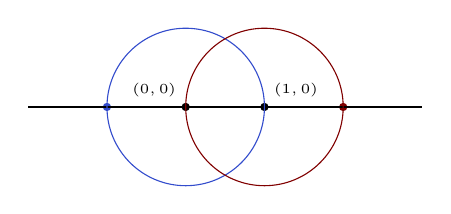
\begin{tikzpicture}
      \node [circ] at (0, 0) {};
      \node [anchor = south east] at (0, 0) {\tiny $(0, 0)$};
      \node [circ] at (1, 0) {};
      \node [anchor = south west] at (1, 0) {\tiny $(1, 0)$};
      \node [mblue] [circ] at (-1, 0) {};
      \node [mred] [circ] at (2, 0) {};

      \draw (-2, 0) -- (3, 0);
      \draw [mblue] circle [radius=1];
      \draw [mred] (1, 0) circle [radius = 1];
    \end{tikzpicture}
  \end{center}
\end{eg}

\begin{defi}[Field of $S$]
  Let $S\subseteq \R^2$ be finite. Define the \emph{field of} $S$ by
  \[
    \Q(S) = \Q(\{\text{coordinates of points in }S\}) \subseteq \R,
  \]
  where we put in the $x$ coordinate and $y$ coordinate separately into the generating set.
\end{defi}
For example, if $S = \{(\sqrt{2}, \sqrt{3})\}$, then $\Q(S) = \Q(\sqrt{2}, \sqrt{3})$.

The key theorem we will use to prove our results is
\begin{thm}[]
  Let $S\subseteq \R^2$ be finite. Then
  \begin{enumerate}
    \item If $R$ is 1-step constructible from $S$, then $[\Q(S\cup \{R\}):\Q(S)] = 1$ or $2$.
    \item If $T\subseteq \R^2$ is finite, $S\subseteq T$, and the points in $T$ are constructible from $S$, Then $[\Q(S\cup T): \Q(S)] = 2^k$ for some $k$ (where $k$ can be $0$).
  \end{enumerate}
\end{thm}

\begin{proof}
  By assumption, there are distinct lines or circles $C, C'$ constructed from $S$ using ruler and compass, such that $R\in C\cap C'$. By elementary geometry, $C$ and $C'$ can be given by the equations
  \begin{align*}
    C&: a(x^2 + y^2) + bx + cy + d = 0,\\
    C'&: a'(x^2 + y^2) + b'x + c'y + d' = 0.
  \end{align*}
  where $a, b, c, d, a', b', c', d' \in \Q(S)$. In particular, if we have a line, then we can take $a = 0$.

  Let $R = (r_1, r_2)$. If $a = a' = 0$ (ie. $C$ and $C'$ are lines), then solving the two linear equations gives $r_1, r_2 \in \Q(S)$. So $[\Q(S\cup \{R\}):\Q(S)] = 1$.

  So we can now assume wlog that $a\not = 0$. We let
  \[
    p = a'b - ab',\quad a'c - ac',\quad \ell = a'd - ad',
  \]
  which are the coefficients when we perform $a'\times C - a \times C'$. Then by assumption, $p \not= 0$ or $q \not= 0$. Otherwise, $c$ and $c'$ would be the same curve. wlog $p \not= 0$. Then since $(r_1, r_2)$ satisfy both equations of $C$ and $C'$, they satisfy
  \[
    px + qy + \ell = 0.
  \]
  In other words, $pr_1 + qr_2 + \ell = 0$. This tells us that
  \[
    r_1 = -\frac{qr_2 + \ell}{p}.\tag{$*$}
  \]
  If we put $r_1, r_2$ into the equations of $C$ and $C'$ and use $(*)$, we get an equation of the form
  \[
    \alpha r_2^2 + \beta r_2  + \gamma = 0,
  \]
  where $\alpha, \beta, \gamma \in \Q(S)$. So we can find $r_2$ (and hence $r_1$ using linear relations) using only a single radical of degree 2. So
  \[
    [\Q(S\cup \{R\}):\Q(S)] = [\Q(S)(r_2): \Q(S)] = 1\text{ or }2,
  \]
  since the minimal polynomial of $r_2$ over $\Q(S)$ has degree 1 or 2.

  Then (ii) follows directly from induction, using the tower law.
\end{proof}

\begin{cor}
  It is impossible to ``double the cube''.
\end{cor}

\begin{proof}
  Consider the cube with unit side length, ie. we are given the set $S = \{(0, 0), (1, 0)\}$. Then doubling the cube would correspond to constructing a side of length $\ell$ such that $\ell^3 = 2$, ie. $\ell = \sqrt[3]{2}$. Thus we need to construct a point $R = (\sqrt[3]{2}, 0)$ from $S$.

  If we can indeed construct this $R$, then we need
  \[
    [\Q(S\cup \{R\}):\Q(S)] = 2^k
  \]
  for some $k$.  But we know that $\Q(S) = \Q$ and $\Q(S\cup \{R\}) = \Q(\sqrt[3]{2})$, and that
  \[
    [\Q(\sqrt[3]{2}):\Q] = 3.
  \]
  This is a contradiction since $3$ is not a power of $2$.
\end{proof}

\section{\texorpdfstring{$K$}{K}-homomorphisms and the Galois Group}
\subsection{\texorpdfstring{$K$}{K}-homomorphisms and the Galois Group}
Usually, we start with a base field $K$, and then add more things on top of it. For example, we start with $\Q$, and then add $\sqrt{2}$ to make $\Q(\sqrt{2})$. We can also add $\sqrt[4]{2}$ to get $\Q(\sqrt[4]{2})$. As usual, we want to consider homomorphisms between the fields $\Q(\sqrt{2})$ and $\Q(\sqrt[4]{2})$. However, we don't want to consider \emph{arbitrary} homomorphisms. We wouldn't want the homomorphisms to touch the things inside the base field $\Q$, or else things would go rather wrong. For example, we will later want to permute the roots of certain polynomials over $\Q$, but it would be bad if that permutation also messed with our lovely, sacred $\Q$. Hence we have the idea of $K$-homomorphisms.

\begin{defi}[$K$-homomorphism]
  Let $K\subseteq L$ and $K\subseteq L'$ be field extensions. A $K$-\emph{homomorphism} $\phi: L \to L'$ is a ring homomorphism such that $\phi|_K = \id$, ie. it fixes everything in $K$. We write $\Hom_K(L, L')$ for the set of all $K$-homomorphisms $L\to L'$.

  A $K$-\emph{isomorphism} is a $K$-homomorphism which is an isomorphism of rings. A $K$-\emph{automorphism} is a $K$-isomorphism $L\to L$. We write $\Aut_K(L)$ for the set of all $K$-automorphism $L\to L$.
\end{defi}
There are a couple of things to take note of
\begin{enumerate}
  \item Given any $\phi \in \Hom_K(L, L')$, we know that
    \begin{enumerate}
      \item Since $\phi|_K = \id$, we know that $\ker \phi \not= L$. Since we know that $\ker \phi$ is an ideal, and a field only has two ideals, we must have $\ker \phi = 0$. So $\phi$ is injective.
      \item $K\subseteq \phi(L)$ is a field extension.
      \item $\phi$ gives an isomorphism $L \to \phi(L)$. So $\phi(L)$ is a field and we get the field extensions $K\subseteq \phi(L) \subseteq L'$.
    \end{enumerate}
  \item If $[L:K] = [L':K] < \infty$, then
    \[
      \{K\text{-homomorphisms}: L \to L'\} = \{K\text{-isomorphisms}: L\to L'\},
    \]
    This is since any $K$-homomorphism $\phi: L\to L'$ is an injection. So $[L:K] = [\phi(L):K]$. Hence we know that $[L':K] = [\phi(L):K]$. But we know that $\phi(L)$ is a subfield of $L'$. This is possible if $L' = \phi(L)$. So $\phi$ is a surjection, and hence an isomorphism.

    In particular, $\Aut_K(L) = \Hom_K(L, L)$.
\end{enumerate}

\begin{eg}
  We want to determine $\Aut_\R(\C)$. If we pick any $\psi\in \Aut_\R(\C)$, then
  \[
    (\psi(\sqrt{-1}))^2 + 1 = \psi(\sqrt{-1}^2 + 1) = \psi(0) = 0.
  \]
  So under any automorphism $\psi$, the image of $\sqrt{-1}$ is a root of $t^2 + 1$. Therefore $\psi(\sqrt{-1}) = \sqrt{-1}$ or $-\sqrt{-1}$. In the first case, $\psi$ is the identity. In the second case, the automorphism is $\phi: a  + b\sqrt{-1} \mapsto a - b\sqrt{-1}$, ie. the complex conjugate. So $\Aut_\R(\C) = \{\id, \phi\}$.

  Similarly, we can show that $\Aut_\Q(\Q(\sqrt{2})) = \{\id, \phi\}$, where $\phi$ swaps $\sqrt{2}$ with $-\sqrt{2}$.
\end{eg}

\begin{eg}
  Let $\mu^3 = 1$ but $\mu \not= 1$ (ie. $\mu$ is a third root of unity). We want to determine $A = \Hom_\Q(\Q(\sqrt[3]{2}), \C)$.

  First define $\phi, \psi$ by
  \begin{align*}
    \phi(\sqrt[3]{2}) &= \sqrt[3]{2}\mu\\
    \psi(\sqrt[3]{2}) &= \sqrt[3]{2}\mu^2,
  \end{align*}
  We have $\phi, \psi \in A$. Are there more?

  Let $\lambda \in A$. Then we must have
  \[
    (\lambda(\sqrt[3]{2}))^3 - 2 = 0.
  \]
  So $\lambda(\sqrt[3]{2})$ is a root of $t^3 - 2$. So it is either $\sqrt[3]{2}, \sqrt[3]{2}\mu$ or $\sqrt[3]{2}\mu^2$. So $\lambda$ is either $\id$, $\phi$ or $\psi$. So $A = \{\id, \phi, \psi\}$.
\end{eg}
Note that in general, if $\alpha$ is algebraic over $\Q$, then $\Q(\alpha) \cong \Q[t]/\bra P_\alpha\ket $. Hence to specify a $\Q$-homomorphism from $\Q(\alpha)$, it suffices to specify the image of $t$, or just the image of $\alpha$.

\begin{defi}[Galois extension]
  Let $K\subseteq L$ be a finite field extension. This is a \emph{Galois extension} if $|\Aut_K(L)| = [L:K]$.
\end{defi}

\begin{defi}[Galois group]
  The \emph{Galois group} of a Galois extension $K\subseteq L$ is defined as $\Gal(L/K) = \Aut_K(L)$. The group operation is defined by function composition. It is easy to see that this is indeed a group.
\end{defi}


\begin{eg}
  The extension $\Q\subseteq \Q(\sqrt{7})$ is Galois. The degree $[\Q(\sqrt{7}):\Q] = 2$, and the automorphism group is $\Aut_\Q(\Q(\sqrt{7})) = \{\id, \phi\}$, where $\phi$ swaps $\sqrt{7}$ with $-\sqrt{7}$.
\end{eg}

\begin{eg}
  The extension $\Q\subseteq \Q(\sqrt[3]{2})$ is not Galois. The degree is $[\Q(\sqrt[3]{2}):\Q] = 3$, but the automorphism group is $\Aut_\Q(\Q(\sqrt[3]{2})) = \{\id\}$.

  To show that there is no other automorphism, note that the automorphism group can be viewed as a subset of $\Hom_\Q(\Q(\sqrt[3]{2}), \C)$. We have just seen that $\Hom_\Q(\Q(\sqrt[3]{2}), \C)$ has three elements, but only the identity maps $\Q(\sqrt[3]{2})$ to itself, while the others map $\sqrt[3]{2}$ to $\sqrt[3]{2}\mu^i \not\in \Q(\sqrt[3]{2})$. So this is the only automorphism.

  The way we should think about this is that there is something missing in $\Q(\sqrt[3]{2})$, namely $\mu$. Without the $\mu$, we cannot get the other automorphisms we need. In fact, in the next example, we will show that $\Q\subseteq \Q(\sqrt[3]{2}, \mu)$ is Galois.
\end{eg}

\begin{eg}
  $\Q\subseteq \Q(\sqrt[3]{2},\mu)$ is a Galois extension. Firstly, we know that $[\Q(\sqrt[3]{2}, \mu): \Q(\sqrt[3]{2})] = 2$ because $\mu^3 - 1 = 0$ implies $\mu^2 + \mu + 1 = 0$. So the minimal polynomial has degree $2$. This also means that $\mu \not\in \Q(\sqrt[3]{2})$. We also know that $[\Q(\sqrt[3]{2}): \Q] = 3$. So we have
  \[
    [\Q(\sqrt[3]{2}, \mu): \Q] = 6
  \]
  by the Tower law.

  Now denote $\alpha = \sqrt[3]{2}$, $\beta = \sqrt[3]{2}\mu$ and $\gamma = \sqrt[3]{2}\mu^2$. Then $\Q(\sqrt[3]{2}, \mu) = \Q(\alpha, \beta, \gamma)$. Now let $\phi \in \Aut_\Q(\Q(\sqrt[3]{2}, \mu))$, then $\phi(\alpha)$, $\phi(\beta)$ and $\phi(\gamma)$ are roots of $t^3 - 2$. These roots are exactly $\alpha, \beta, \gamma$. So
  \[
    \{\phi(\alpha), \phi(\beta), \phi(\gamma)\} = \{\alpha, \beta, \gamma\}.
  \]
  Hence $\phi$ is completely determined by a permutation of the roots of $t^3 - 2$. So $\Aut_\Q(\sqrt[3]{2}, \mu) \cong S_3$ and $|\Aut_\Q(\sqrt[3]{2}, \mu)| = 6$.
\end{eg}

One of the goals of this course is to prove the \emph{Fundamental theorem of Galois theory}, which roughly says: if $K\subseteq L$ is a finite Galois extension, then there is a one-to-one correspondence of the set of subgroups $H\leq \Gal(L/K)$ and the intermediate fields $K\subseteq F \subseteq L$. In particular, the normal subgroups corresponds to the ``normal extensions'', which is something we will define later.

The theorem actually says even more than this, but we will get to those when we actually reach the fundamental theorem.

\subsection{Splitting fields}
\begin{notation}
  Let $K\subseteq L$ be a field extension, $f\in K[t]$. We write $\Root_f(L)$ for the roots of $f$ in $L$.
\end{notation}

\begin{lemma}
  Let $K\subseteq L$ be a field extension, $f\in K[t]$ irreducible, $\deg f > 0$. Then there is a 1-to-1 correspondence between $\Root_f(L)$ and $\Hom_K(K[t]/\bra f\ket, L)$.
\end{lemma}

\begin{proof}
  Since $f$ is irreducible, $\bra f\ket$ is a maximal ideal. So $K[t] / \bra f\ket$ is a field. Also there is a natural inclusion $K\subseteq K[t] / \bra f\ket$. So it makes sense to talk about $\Hom_K(K[t]/\bra f\ket, L)$.

  To any $\beta\in \Root_f(L)$, we assign $\phi: K[t]/\bra f\ket \to L$ where we map $\bar t \mapsto \beta$ ($\bar t$ is the equivalence class of $t$). This is well defined since if $\bar{t} = \bar{g}$, then $g = t + hf$ for some $h \in K[t]$. So $\phi(\bar{g}) = \phi(\overline{t + hf}) = \beta + h(\beta) f(\beta) = \beta$.

  Conversely, given any $K$-homomorphism $\phi: K[t]/\bra f\ket \to L$, we assign $\beta = \phi(\bar t)$. This is a root since $f(\beta) = f(\phi(\bar t)) = \phi(f(\bar t)) = \phi(0) = 0$.

  This assignments are inverses to each other. So we get a one-to-one correspondence.
\end{proof}
Note that we have previously said that if $K\subseteq F$ is a field extension, then for any $\alpha\in F$ with minimal polynomial $P_\alpha$, we have $K[t]/\bra P_\alpha\ket \cong K(\alpha)$. Since an irreducible $f$ is minimal polynomial of its roots, we can view the above lemma as telling us something about $\Hom_K(K(\alpha), L)$.

\begin{cor}
  Let $K\subseteq L$ be a field extension, $f \in K[t]$ irreducible, $\deg f > 0$. Then
  \[
    \left| \Hom_K(K[t]/\bra f\ket, L) \right| \leq \deg f.
  \]
  In particular, if $E = K[t]/\bra f\ket$, then
  \[
    |\Aut_K(E)| = |\Root_f(E)| \leq \deg f = [E:K].
  \]
  So $K \subseteq E$ is a Galois extension iff $|\Root_f(E)| = \deg f$.
\end{cor}

\begin{proof}
  This follows directly from the following three facts:
  \begin{itemize}
    \item $|\Root_f(L)| \leq \deg f$
    \item $\Aut_K(E) = \Hom_K(E, E)$
    \item $\deg f = [K(\alpha): K] = [E:K]$.
  \end{itemize}
\end{proof}

\begin{defi}[Splitting field]
  Let $K\subseteq L$ be a field extensions, $f\in K[t]$. We say $f$ \emph{splits} over $L$ if
  \[
    f = a(t - \alpha_1)\cdots (t - \alpha_n)
  \]
  for some $a \in K$ and $\alpha_j \in L$, ie. we can factorize it into a product of linear terms. Alternatively, this says that $L$ contains all roots of $f$.

  We say $L$ is a \emph{splitting field} of $f$ if $L = K(\alpha_1, \cdots, \alpha_n)$. This is the smallest field where $f$ has all its roots.
\end{defi}

\begin{eg}\leavevmode
  \begin{itemize}
    \item $\C$ is the splitting field of $t^2 + 1 \in \R[t]$.
    \item $\Q(\sqrt[3]{2}, \mu)$ is a splitting field of $t^3 - 2 \in \Q[t]$, where $\mu$ is a third root of unity.
    \item By the fundamental theorem of algebra, for any $K\subseteq \C$ and $f\in K[t]$, there is a splitting field $L\subseteq \C$ of $f$.
  \end{itemize}
\end{eg}

\begin{thm}
  Let $K$ be a field, $f\in K[t]$. Then
  \begin{enumerate}
    \item There is a splitting field of $f$.
    \item The splitting field is unique (up to $K$-isomorphism).
  \end{enumerate}
\end{thm}

\begin{proof}\leavevmode
  \begin{enumerate}
    \item If $\deg f = 0$, then $K$ is a splitting field of $f$. So we can assume $\deg f > 0$.

      Pick $g | f$ in $K[t]$, where $g$ is irreducible and $\deg g > 0$. We have the field extension $K\subseteq K[t]/\bra g\ket$. Let $\alpha_1 = \bar t$. Then $g(\alpha_1) = 0$ which implies that $f(\alpha_1) = 0$. Hence we can write $f = (t - \alpha_1) h$ in $K(\alpha_1)[f]$. Note that $\deg h < \deg f$. So we can repeat the process on $h$ iteratively to get a field extensions $K\subseteq K(\alpha_1, \cdots, \alpha_n)$. This $K(\alpha_1, \cdots, \alpha_n)$ is a splitting field of $f$.

    \item Assume $L$ and $L'$ are both splitting fields of $f$ over $K$. We want to find a $K$-isomorphism from $L$ to $L'$.

      Pick largest $F, F'$ such that $K \subseteq F\subseteq L$ and $K\subseteq F' \subseteq L'$ are field extensions and there is a $K$-isomorphism from $\psi: F \to F'$. By ``largest'', we mean we want to maximize $[F:K]$.

      We want to show that we must have $F = L$. Then we are done because this means that $F'$ is a splitting field, and hence $F' = L'$.

      So suppose $F\not= L$. We will try to produce a larger $\tilde{F}$ with $K$-isomorphism $\tilde{F} \to \tilde{F}' \subseteq L'$.

      Since $F\not= L$, we know that there is some $\alpha \in \Root_f(L)$ such that $\alpha\not\in F$. Then there is some irreducible $g\in K[t]$ with $\deg g > 0$ such that $g(\alpha) = 0$ and $g | f$. Say $f = gh$.

      Now we know that there is an isomorphism $F[t]/\bra g\ket \to F(\alpha)$ by $\bar t \mapsto \alpha$. The isomorphism $\psi: F \to F'$ extends to a isomorphism $\mu: F[t] \to F'[t]$. Then since the coefficients of $f$ are in $K$, we have  $f = \mu(f) = \mu(g)\mu(h)$.  So $\mu(g) | f$ in $F'[t]$. Since $g$ is irreducible in $F[t]$, $\mu(g)$ is irreducible in $F'[t]$. So by the previous proposition, there is some $\alpha' \in \Root_{\mu(g)}(L') \subseteq \Root_f(L')$ and isomorphism $F'[t]/\bra \mu(g)\ket \to F'(\alpha')$.
      Now $\mu$ induces a $K$-isomorphism $F[t]/\bra g\ket \to F[t]/\bra \mu(g)\ket$, which in turn induces a $K$-isomorphism $F(\alpha) \to F'(\alpha)$. This contradicts the maximality of $F$. So we must have had $F = L$.
  \end{enumerate}
\end{proof}
Note that the splitting is unique just up to isomorphism. We could be quotienting by different polynomials and still get the same splitting field.
\begin{eg}
  $\Q(\sqrt{7})$ is a splitting field of $t^2 - 7\in \Q[t]$. At the same time, $\Q(\sqrt{7})$ is also a splitting field of $t^2 + 3t + \frac{1}{2} \in \Q[t]$.
\end{eg}
\subsection{Algebraic closures}

\begin{defi}[Algebraically closed field]
  A field $L$ is \emph{algebraically closed} if for all $g\in L[t]$, we have
  \[
    f = a(t - \alpha_1)(t - \alpha_2) \cdots (t - \alpha_n)
  \]
  for some $a, \alpha_i \in L$.

  Assume $K\subseteq L$ is a field extension. We say $L$ is an algebraic closure of $K$ if
  \begin{itemize}
    \item $L$ is algebraic over $K$
    \item $L$ is algebraically closed.
  \end{itemize}
\end{defi}

\begin{eg}
  $L$ be an algebraically closed field iff all $f\in L[t]$ has a root iff ($L\subseteq E$ is a finite extension implies $E = L$)
\end{eg}
The last ``if and only if'' is because if $L \subseteq E$ is finite, then $E$ is algebraic over $L$, and hence must be $L$.

\begin{eg}
  $\C$ is algebraically closed by the fundamental theorem of algebra, and is the algebraic closure of $\R$ (but not $\Q$).
\end{eg}

Before we prove our next theorem, we need the following lemma:
\begin{lemma}
  If $R$ is a commutative ring, then it has a maximal ideal. In particular, if $I$ is an ideal of $R$, then there is a maximal ideal that contains $I$.
\end{lemma}

\begin{proof}
  Let
  \[
    \mathcal{P} = \{I: I\text{ is an ideal of }R, I \not= R\}.
  \]
  If $I_1 \subseteq I_2 \subseteq \cdots$ is any chain of $I_i \in P$, then $I = \bigcup I_i \in \mathcal{P}$. By Zorn's lemma, there is a maximal element of $\mathcal{P}$ (containing $I$). So $R$ has at least one maximal ideal (containing $I$).
\end{proof}

\begin{thm}[Existence of algebraic closure]
  Any field $K$ has an algebraic closure.
\end{thm}

\begin{proof}
  Let
  \[
    \mathcal{A} = \{\lambda = (f, j): f\in K[t] \text{ irreducible monic}, 1 \leq j \leq \deg f\}.
  \]
  We can think of $j$ as labelling which root of $f$ we want. For each $\lambda \in \mathcal{A}$, we assign a variable $t_\lambda$. We take
  \[
    R = K[t_\lambda: \lambda \in \mathcal{A}]
  \]
  to be the polynomial ring over $K$ with variables $t_\lambda$. This $R$ contains all the ``roots'' of the polynomials in $K$. However, we've got a bit too much. For example, (if $K = \Q$), in $R$, $\sqrt{3}$ and $\sqrt{3} + 1$ would be put down as separate, unrelated variables. So we want to quotient this $R$ by something.

  For every monic and irreducible $f \in K[t]$, we define
  \[
    \tilde{f} = f  - \prod_{j = 1}^{\deg f} (t - t_{(f, j)}) \in R[t].
  \]
  Denote the coefficient of $t^\ell$ in $\tilde{f}$ by $b_{(f, \ell)}$. For example, let $f = t^2 - 2 \in \Q[t]$. Then
  \[
    \tilde{f} = (t^2 - 2) - (t - t_{(f, 1)})(t - t_{(f, 2)}) = (t_{(f, 1)} + t_{(f, 2)})t - (t_{(f, 1)}t_{(f, 2)} + 2).
  \]
  Intuitively, we should think of $t_{(f, 1)}$ and $t_{(f, 2)}$ as $\pm \sqrt{2}$. Then we \emph{should} have $t_{(f, 1)} + t_{(f, 2)} = t_{(f, 1)}t_{(f, 2)} + 2 = 0$. We see that we want to declare the coefficients of $t$ and $1$ as zero.

  To do so, let $I\subseteq R$ be the ideal generated by all such coefficients. We now want to quotient $R$ by $I$. We first have to check that $I\not= R$.

  Suppose not. So there are $b_{(f_1, \ell_1)}, \cdots, b_{(f_r, \ell_r)}$ with $g_1, \cdots, g_r \in R$ such that
  \[
    g_1 b_{(f_1, \ell_1)} + \cdots + g_r b_{(f_r, \ell_r)} = 1.\tag{$*$}
  \]
  We will attempt to reach a contradiction by constructing a homomorphism $\phi$ that sends each $b_{(f_i, \ell_i)}$ to $0$.

  Let $E$ be a splitting field of $f_1f_2\cdots f_r$. So in $E[t]$, for each $i$, we can write
  \[
    f_i = \prod_{j = 1}^{\deg f_i} (t - \alpha_{i, j}).
  \]
  Then we define a homomorphism $\phi: R \to E$ by
  \[
    \begin{cases}
      \phi(t_{(f_i, j)}) = \alpha_{i, j}\\
      \phi(t_\lambda) = 0 & \text{otherwise}
    \end{cases}
  \]
  This induces a homomorphism $\tilde{\phi}: R[t] \to E[t]$.

  Now apply
  \begin{align*}
    \tilde{\phi}(\tilde{f}_i) &= \tilde{\phi}(f_i) - \prod_{j = 1}^{\deg f_i} \tilde{\phi}(t - t_{(f_i, j)})\\
    &= f_i - \prod_{j = 1}^{\deg f_i} (t - \alpha_{i, j})\\
    &= 0
  \end{align*}
  So $\phi(b_{(f_i, \ell_i)}) = 0$ as $b_{(f_i, \ell_i)}$ is a coefficient of $f_i$.

  Now we apply $\phi$ to $(*)$ to obtain
  \[
    \phi(g_1 b_{(f_1, \ell_1)} + \cdots + g_r b_{(f_r, \ell_r)}) = \phi(1).
  \]
  But this is a contradiction since the left had side is $0$ while the right is $1$. Hence we must have $I \not= R$.

  We would like to quotient by $I$, but we have to be a bit more careful, since the quotient need not be a field. Instead, pick a maximal ideal $M$ containing $I$, and consider $L = R/M$. Then $L$ is a field. Moreover, since we couldn't have quotiented out anything in $K$ (any ideal containing anything in $K$ would automatically contain all of $R$), this is a field extension $K\subseteq L$. We want to show that $L$ is an algebraic extension.

  Now we show that $L$ is algebraic over $K$. First we pick $\alpha\in L$. Since $L = R/M$ and $R$ is generated by the terms $t_{\lambda}$, there is some $(f_1, j_1) ,\cdots, (f_r, j_r)$ such that
  \[
    \alpha \in K(\bar{t}_{(f_i, j_i)}, \cdots, \bar{t}_{(f_r, j_r)}).
  \]
  So $\alpha$ is algebraic over $K$ if each $\bar{t}_{(f_i, j_i)}$ is algebraic over $K$. To show this, note that $\tilde{f}_i = 0$, since we've quotiented out each of its coefficients. So by definition,
  \[
    0 = f_i(t) - \prod_{j = 1}^{\deg f_i} (t - \bar{t}_{(f_i, j)}).
  \]
  So $f_i(\bar{t}_{(f_i, j_i)}) = 0$. So done.

  Finally, we have to show that $L$ is algebraically closed. Suppose $L\subseteq E$ is a finite (and hence algebraic) extension. We want to show that $L = E$.

  Consider arbitrary $\beta \in E$. Then $\beta$ is algebraic over $L$, say a root of $f\in L[t]$. Since every coefficient of $f$ can be found in some finite extension $K(\bar{t}_{(f_i, j_i)}, \cdots, \bar{t}_{(f_r, j_r)})$, there is a finite extension $F$ of $K$ that contains all coefficients of $f$. Since $F(\beta)$ is a finite extension of $F$. So $F(\beta)$ is a finite and hence algebraic extension of $K$. In particular, $\beta$ is algebraic in $K$.

  Let $P_\beta$ be the minimal polynomial of $\beta$ over $K$. Since all polynomials in $K$ split over $L$ by construction ($f(t) = \prod (t - \bar{t}_{(f, j)})$), its roots must in $L$. In particular, $\beta \in L$. So $L = E$.
\end{proof}

\begin{thm}[Uniqueness of algebraic closure]
  Any field $K$ has a unique algebraic closure up to $K$-isomorphism.
\end{thm}

To prove this, we will use Zorn's lemma. Given algebraic closures $L, L'$, we want to be able to define an isomorphism between $L$ and $L'$. This is hard, since $L$ and $L'$ are big scary things. What we do know is how to define an isomorphism between $K\subseteq L$ and $K\subseteq L'$ (in the trivial way). Also, if we have an isomorphism between $F\subsetneq L$ and $F'\subsetneq L'$, we can extend this to slightly bigger subsets of $L$ and $L'$. Of course, we can repeat this process and get isomorphisms between bigger and bigger subsets of $L$ and $L'$, but there is no guarantee that we will actually reach $L$ and $L'$ themselves in finite time. Hence we use Zorn's lemma to ``cheat'' and jump to the end at once, and get an isomorphism between $L$ and $L'$.

\begin{proof}(sketch)
  Suppose $L, L'$ are both algebraic closures of $K$. Let
  \[
    \mathcal{H} = \{(F, \psi): K\subseteq F\subseteq L, \psi \in \Hom_K(F, L')\}.
  \]
  We define a partial order on $\mathcal{H}$ by $(F_1, \psi_1) \leq (F_2, \psi_2)$ and $\psi_1= \psi_2|_{f_1}$.

  We have to show that chains have upper bounds. Given chain $\{(F_\alpha, \psi_\alpha)\}$, we define
  \[
    F = \bigcup F_\alpha,\quad \psi(x) = \psi_\alpha(x)\text{ for }x \in F_\alpha.
  \]
  Then $(F, \psi) \in \mathcal{H}$. Then applying Zorn's lemma, there is a maximal element of $\mathcal{H}$, say $(F, \psi)$. The final part is to prove that $F = L$, and that $\phi(L) = L'$, which is left as an exercise. This proof uses the idea of ideals, similar to what we did to show splitting fields are unique.
  % complete
\end{proof}

\subsection{Separable extensions}
The notion of separable extensions is rather important. Among all things, we need it for the fundamental theorem of Galois theory. Before we can get to it, we need some preparations first. We first define what it means for a \emph{polynomial} to be separable.

\begin{defi}[Separable polynomial]
  Let $K$ be a field, $f\in K[t]$ non-zero, and $L$ a splitting field of $f$. For an irreducible $f$, we say it is \emph{separable} if $f$ has no repeated roots, ie. $|\Root_f(L)| = \deg f$. For a general polynomial $f$, we say it is \emph{separable} if all its irreducible factors in $K[t]$ are separable.
\end{defi}

\begin{eg}
  Any linear polynomial $t - a$ (with $a \in K$) is separable.
\end{eg}
This is, however, not a very interesting example. To get to more interesting examples, we need even more preparation.

\begin{defi}[Formal derivative]
  Let $K$ be a field, $f \in K[t]$. \emph{(Formal) differentiation} is a $K$-linear map $K[t] \to K[t]$ defined by $t^n \mapsto n t^{n - 1}$, where $n = 1 + 1 + \cdots + 1$ ($n$ times).

  The image of a polynomial $f$ is the \emph{derivative} of $f$, written $f'$.
\end{defi}
This is similar to how we differentiate real or complex polynomials.

The following lemma summarizes the properties of the derivative we need.
\begin{lemma}
  Let $K$ be a field, $f, g\in K[t]$. Then
  \begin{enumerate}
    \item $(f + g)' = f' + g'$, $(fg)' = fg' + f'g$.
    \item Assume $f \not= 0$ and $L$ is a splitting field of $f$. Then $f$ has a repeated root in $L$ if and only if $f$ and $f'$ have a common (non-constant) irreducible factor in $K[t]$ (if and only if $f$ and $f'$ have a common root in $L$).
  \end{enumerate}
\end{lemma}
This will allow us to show when irreducible polynomials are separable.

\begin{proof}\leavevmode
  \begin{enumerate}
    \item $(f + g)' = f' + g'$ is true by linearity.

      To show that $(fg)' = fg' + f'g$, we use linearity to reduce to the case where $f = t^n, g = t^m$. Then both sides are $(n + m) t^{n + m - 1}$. So this holds.
    \item First assume that $f$ has a repeated root. So let $f = (t - \alpha)^2 h \in L[t]$ where $\alpha \in L$. Then $f' = 2(t - \alpha)h + (t - \alpha)^2 h' = (t - \alpha)(2h + (t - \alpha)h')$. So $f(\alpha) = f'(\alpha) = 0$. So $f$ and $f'$ have common roots. However, we want a common irreducible factor in $K[t]$, not $L[t]$. So we let $P_\alpha$ be the minimal polynomial of $\alpha$ over $K$. Then $P_\alpha | f$ and $P_\alpha | f'$.

    Now suppose $e$ is a common irreducible factor of $f$ and $f'$ in $K[t]$, with $\deg e > 0$. Pick $\alpha \in \Root_e(L)$. Then $\alpha \in \Root_f(L) \cap \Root_{f'}(L)$.

      Since $\alpha$ is a root of $f$, we can write $f = (t - \alpha)q \in L[t]$ for some $q$. Then
      \[
        f' = (t - \alpha) q' + q.
      \]
      Since $(t - \alpha) | f'$, we must have $(t - \alpha) | q$. So $(t - \alpha)^2 | f$.
  \end{enumerate}
\end{proof}

Recall that the characteristic of a field $\Char K$ is the minimum $p$ such that $p \cdot 1_K = 0$. If no such $p$ exists, we say $\Char K = 0$. For example, $\Q$ has characteristic $0$ while $\Z_p$ has characteristic $p$.
\begin{cor}
  Let $K$ be a field, $f \in K[t]$ non-zero irreducible. Then
  \begin{enumerate}
    \item If $\Char K = 0$, then $f$ is separable.
    \item If $\Char K = p > 0$, then $f$ is not separable iff $\deg f > 0$ and $f \in K[t^p]$.  For example, $t^{2p} + 3t^p + 1$ is not separable.
  \end{enumerate}
\end{cor}
\begin{proof}
  By definition, for irreducible $f$, $f$ is not separable iff $f$ has a repeated root. So by our previous lemma, $f$ is not separable if and only if $f$ and $f'$ have a common irreducible factor of positive degree in $K[t]$. However, since $f$ is irreducible, its only factors are $1$ and itself. So this can happen if and only if $f' = 0$.

  To make it more explicit, we can write
  \[
    f = a_n t^n + \cdots + a_1 t + a_0.
  \]
  Then we can write
  \[
    f' = n a_n t^{n - 1} + \cdots + a_1.
  \]
  Now $f' = 0$ if and only if all coefficients $i a_i = 0$ for all $i$.
  \begin{enumerate}
    \item Suppose $\Char K = 0$, then if $\deg f = 0$, then $f$ is trivially separable. If $\deg f > 0$, then $f$ is not separable iff $f' = 0$ iff $i a_i = 0$ for all $i$ iff $a_i = 0$ for $i \geq 1$. But we cannot have a polynomial of positive degree with all its coefficients zero (apart from the constant term). So $f$ must be separable.
    \item If $\deg f = 0$, then $f$ is trivially separable. So assume $\deg f > 0$.

      Then $f$ is not separable $\Leftrightarrow$ $f' = 0$ $\Leftrightarrow$ $i a_i = 0$ for $i \geq 0$ $\Leftrightarrow$ $a_i = 0$ for all $i \geq 1$ not multiples of $p$ $\Leftrightarrow$ $f \in K[t^p]$.
  \end{enumerate}
\end{proof}
Using this, it should be easy to find lots of examples of separable polynomials.

\begin{defi}[Separable elements and extensions]
  Let $K \subseteq L$ be an algebraic field extension. We say $\alpha \in L$ is \emph{separable} over $K$ if $P_\alpha$ is separable, where $P_\alpha$ is the minimal polynomial of $\alpha$ over $K$.

  We say $L$ is \emph{separable} over $K$ (or $L\subseteq L$ is \emph{separable}) if all $\alpha \in L$ are separable.
\end{defi}

\begin{eg}\leavevmode
  \begin{itemize}
    \item The extensions $Q \subseteq \Q(\sqrt{2})$ and $\R \subseteq \C$ are separable because $\Char \Q = \Char \R = 0$. So we can apply our previous corollary.
    \item Let $L = \F_p(s)$ be the field of rational functions in $s$ over $\F_p$ (which is the fraction field of $\F_p[s]$), and $K = \F_p(s^p)$. We have $K \subseteq L$, and $L = K(s)$. Since $s^p \in K$, $s$ is a root of $t^p - s^p \in K[t]$.  So $s$ is algebraic over $K$ and hence $L$ is algebraic over $K$. In fact $P_s = t^p - s^p$ is the minimal polynomial of $s$ over $K$.

      Now $t^p - s^p = (t - s)^p$ since the field has characteristic $p$. So $\Root_{t^p - s^p}(L) = \{s\}$. So $P_s$ is not separable.
  \end{itemize}
\end{eg}
So we now have separable polynomials and separable extensions, and we have many examples of these. But why do we care? Eventually, our goal is to show that if $K\subseteq L$ is a finite separable extension, then $K \subseteq L$ is simple, ie. $L = K(\alpha)$ for some $\alpha \in L$. This is a really nice and useful result.

\begin{eg}
  Consider $\Q \subseteq \Q(\sqrt{2}, \sqrt{3})$. This is a separable finite extension. So we should be able to generate $\Q(\sqrt{2}, \sqrt{3})$ by just one element, not just two. In fact, we can use $\alpha = \sqrt{2} + \sqrt{3}$, since we have
  \[
    \alpha^3 = 11\sqrt{2} + 9\sqrt{3} = 2\sqrt{2} + 9 \alpha.
  \]
  So since $\alpha^3 \in \Q(\alpha)$, we know that $\sqrt{2} \in \Q(\alpha)$. So we also have $\sqrt{3} \in \Q(\alpha)$.
\end{eg}
In general, it is not easy to find an $\alpha$ that works, but we our later result will show that such an $\alpha$ exists.

\begin{lemma}
  Let $K\subseteq F\subseteq L$ be finite extensions, and $K\subseteq E$ be a field extension. Then for all $\alpha \in L$, we have
  \[
    |\Hom_K(F(\alpha), E)|| \leq [F(\alpha): F] |\Hom_K(F, E)|.
  \]
\end{lemma}
Note that if $P_\alpha$ is the minimal polynomial of $\alpha$ over $F$, then $[F(\alpha): F] = \deg P_\alpha$. So we can interpret this intuitively as follows: for each $\psi \in \Hom_K(F, E)$, we can obtain a $K$-homomorphism in $\Hom_K(F(\alpha), E)$ by sending things in $F$ according to $\psi$, and then send $\alpha$ to any root of $P_\alpha$. Then there are at most $[F(\alpha): F]$ $K$-homomorphisms generated this way. Moreover, each $K$-homomorphism in $\Hom_K(F(\alpha), E)$ can be created this way. So we get this result.

\begin{proof}
  We show that for each $\psi \in \Hom_K(F, E)$, there are at most $[F(\alpha):F]$ $K$-isomorphisms in $\Hom_K(F(\alpha), E)$ that restrict to $\psi$ in $F$. Since each $K$-isomorphism in $\Hom_K(F(\alpha), E)$ has to restrict to something, it follows that there are at most $[F(\alpha): F] |\Hom_K(F, E)|$ $K$-homomorphisms from $F(\alpha)$ to $E$.

  Now let $P_\alpha$ be the minimal polynomial for $\alpha$ in $F$, and let $\psi \in \Hom_K(F, E)$. We want to show that there is a one-to-one correspondence between the roots of $P_\alpha$ in $E$ and the homomorphisms $\{\phi \in \Hom_K(F(\alpha), E): \phi|_F = \psi\}$. Except that the previous sentence makes no sense, since $P_\alpha \in F[t]$ but we are not told that $F$ is a subfield of $E$. So we use our $\psi$ to ``move'' our things to $E$.

  We let $M = \psi(F) \subseteq E$, and $q \in M[t]$ be the image of $P_\alpha$ under the homomorphism $F[t] \to M[t]$ induced by $\psi$. As we have previously shown, there is a one-to-one correspondence
  \[
    \Root_q(E) \longleftrightarrow \Hom_M(M[t]/\bra q \ket, E).
  \]
  What we really want to show is the correspondence between $\Root_q(E)$ and the $K$-homomorphisms $F[t]/\bra P_\alpha\ket \to E$ that restrict to $\psi$ on $F$. Let's ignore the quotient for the moment and think: what does it mean for $\phi \in \Hom_K(F[t], E)$ to restrict to $\psi$ on $F$? We know that any $\phi \in \Hom_L(F[t], E)$ is uniquely determined by the values it takes on $F$ and $t$. Hence if $\phi|_F = \psi$, then our $\phi$ must send $F$ to $\psi(F) = M$, and can send $t$ to anything in $E$. This corresponds exactly to the $M$-homomorphisms $M[t] \to E$ that does nothing to $M$ and sends $t$ to that ``anything'' in $E$.

  The situation does not change when we put back the quotient. Changing from $M[t] \to E$ to $M[t]/\bra q\ket \to E$ just requires that the image of $t$ must be a root of $q$. On the other hand, using $F[t]/\bra P_\alpha\ket$ instead of $F[t]$ requires that $\phi(P_\alpha(t)) = 0$. But we know that $\phi(P_\alpha) = \psi(P_\alpha) = q$. So this just requires $q(t) = 0$ as well. So we get the one-to-one correspondence
  \[
    \Hom_M(M[t]/\bra q \ket, E) \longleftrightarrow \{\phi \in \Hom_K(F[t]/\bra P_\alpha \ket, E): \phi|_F = \psi\}.
  \]
  Since $F[t]/\bra P_\alpha\ket = F(\alpha)$, there is a one-to-one correspondence
  \[
    \Root_q(E) \longleftrightarrow \{\phi \in \Hom_K(F(\alpha), E): \phi|_F = \psi\}.
  \]
  So done.
\end{proof}

\begin{thm}[]
  Let $K\subseteq F\subseteq L$ be a finite extension, $K\subseteq E$ a field extension. Then
  \begin{enumerate}
    \item $|\Hom_K(L, E)| \leq [L:K]$
    \item If equality holds in (i), then
      \begin{enumerate}
        \item $|\Hom_K(F, E)| = [F:K]$.
        \item The map $\Hom_K(L, E) \to \Hom_K(F, E)$ be restriction is surjective.
      \end{enumerate}
  \end{enumerate}
\end{thm}

\begin{proof}\leavevmode
  \begin{enumerate}
    \item We have previously shown that there is some $K\subseteq F_i \subseteq L$ such that $K = F_0 \subseteq F_1 \subseteq\cdots \subseteq F_n = L$, and for each $i$, there is some $\alpha_i$ such that $F_i = F_{i - 1}(\alpha_i)$. Then by our previous lemma, we have
      \begin{align*}
        |\Hom_K(L, E)| &\leq [F_n:F_{n - 1}] |\Hom_K(F_{n - 1}, E)|\\
        &\leq [F_n: F_{n - 1}][F_{n - 1}: F_{n - 2}] |\Hom_K(F_{n - 2}, E)|\\
        &\quad \vdots\\
        &\leq [F_n:F_{n - 1}][F_{n - 1}:F_{n - 2}] \cdots [F_1:F_0] |\Hom_K(F_0, E)|\\
        &= [F_n:F_0]\\
        &= [L:K]
      \end{align*}
    \item
    \begin{enumerate}
      \item If equality holds in (i), then every inequality in the proof above has to an equality. If we pick that $\alpha_i$ carefully, we can assume that $F = F_i$ for some $i$. Then we get
        \[
          |\Hom_K(L, E)| = [L:F] |\Hom_K(F, E)| = [L:K].
        \]
        Then the tower law says
        \[
          |\Hom_K(F, E)| = [F:K].
        \]
      \item By the proof of the lemma, for each $\psi \in \Hom_K(F, E)$, we know that
        \[
          \{\phi: \Hom_K(L, E): \phi|_F = \psi\} \leq [L:F].\tag{$*$}
        \]
        As we know that
        \[
          |\Hom_K(F, E)| = [F:K],\quad |\Hom_K(L, E)| = [L:K]
        \]
        we must have had equality in $(*)$, or else we won't have enough elements. So in particular $\{\phi: \Hom_K(L, E): \phi|_F = \psi\} \geq 1$. So the map is surjective.
    \end{enumerate}
  \end{enumerate}
\end{proof}

\begin{thm}[]
  Let $K\subseteq L$ be a finite field extension. Then the following are equivalent:
  \begin{enumerate}
    \item There is some extension $E$ of $K$ such that $|\Hom_K(L, E)| = [L:K]$
    \item $K\subseteq L$ is separable.
    \item $L = K(\alpha_1, \cdots, \alpha_n)$ such that $P_{\alpha_i}$, the minimal polynomial of $\alpha_i$ over $K$, is separable for all $i$.
    \item $L = K(\alpha_1, \cdots, \alpha_n)$ such that $R_{\alpha_i}$, the minimal polynomial of $\alpha_i$ over $K(\alpha_1, \cdots, \alpha_{i - 1})$ is separable for all $i$ for all $i$.
  \end{enumerate}
\end{thm}

\begin{proof}\leavevmode
  \begin{itemize}
    \item (i) $\Rightarrow$ (ii): For all $\alpha \in L$, if $P_\alpha$ is the minimal polynomial of $\alpha$ over $K$, then since $K(\alpha)$ is a subfield of $L$, by our previous theorem, we have
      \[
        |\Hom_K(K(\alpha), E)| = [K(\alpha): K].
      \]
      We also know that $|\Root_{P_\alpha}(E)| = |\Hom_K(K(\alpha), E)|$, and that $[K(\alpha): K] = \deg P_\alpha$. So we know that $P_\alpha$ has no repeated roots in any splitting field. So $P_\alpha$ is a separable. So $K\subseteq L$ is a separable extension.
    \item (ii) $\Rightarrow$ (iii): Obvious from definition
    \item (iii) $\Rightarrow$ (iv): Note that since $R_{\alpha_i}$ is a minimal polynomial in $K(\alpha_1, \cdots, \alpha_{i - 1})$, we know that $R_{\alpha_i} | P_{\alpha_i}$. So $R_{\alpha_i}$ is separable as $P_{\alpha_i}$ is separable.
    \item (iv) $\Rightarrow$ (i): Let $E$ be the splitting field of $P_{\alpha_1}, \cdots, P_{\alpha_n}$. We do induction on $n$ to show that this satisfies the properties we want. If $n = 1$, then $L = K(\alpha_1)$. Then we have
      \[
        |\Hom_K(L, E)| = |\Root_{P_{\alpha_i}}(E)| = \deg P_{\alpha_1} = [K(\alpha_1): K] = [L:K].
      \]
      We now induct on $n$. So we can assume that (iv) $\Rightarrow $ (i) holds for smaller number of generators. For convenience, we write $K_i = K(\alpha_1, \cdots, \alpha_i)$. Then we have
      \[
        |\Hom_K(K_{n - 1}, E)| = [K_{n - 1}: K].
      \]
      We also know that
      \[
        |\Hom_K(K_n, E)| \leq [K_n: K_{n - 1}] |\Hom_K(K_{n - 1}, E)|.
      \]
      What we actually want is equality. We now re-do (parts of) the proof of this result, and see that separability guarantees that equality holds. If we pick $\psi \in \Hom_K(K_{n - 1}, E)$, then there is a one-to-one correspondence between $\{\phi \in \Hom_K(K_n, E): \phi|_{K_{n - 1}} = \psi\}$ and $\Root_q(E)$, where $q \in M[t]$ is defined as the image of $R_{\alpha_n}$ under $K_{n - 1}[t] \to M[t]$, and $M$ is the image of $\psi$.

      Since $P_{\alpha_n} \in K[t]$ and $R_{\alpha_n} | P_{\alpha_n}$, then $q | P_{\alpha_n}$. So $q$ splits over $E$. By separability assumption , we get that
      \[
        |\Root_q(E)| = \deg q = \deg R_{\alpha_n} = [K_n: K_{n - 1}].
      \]
      Hence we know that
      \begin{align*}
        |\Hom_K(L, E)| &= [K_n): K_{n - 1}] | \Hom_K(K_{n - 1}, E)|\\
        &= [K_n: K_{n - 1}][K_{n - 1}: K]\\
        &= [K_n: K].
      \end{align*}
      So done.
  \end{itemize}
\end{proof}

We will need a rather helpful lemma. This will allow us to prove a small part of the primitive element theorem, but will be much more useful later on.
\begin{lemma}
  Let $L$ be a field, $L^*\setminus \{0\}$ be the multiplicative group of $L$. If $G$ is a finite subgroup of $L^*$, then $G$ is cyclic.
\end{lemma}

\begin{proof}
  Since $L^*$ is abelian, $G$ is also abelian. Then by the structure theorem on finite abelian groups,
  \[
    G \cong \frac{Z}{\bra n_1\ket} \times \cdots \times \frac{\Z}{\bra n_r\ket},
  \]
  for some $n_i \in \N$. Let $m$ be the least common multiple of $n_1, \cdots, n_r$, and let $f = t^m - 1$.

  If $\alpha \in G$, then $\alpha^m = 1$. So $f(\alpha) = 0$ for all $\alpha \in G$. Therefore
  \[
    |G| = n_1 \cdots n_r \leq |\Root_f(L)| \leq \deg f = m.
  \]
  Since $m$ is the least common multiple of $n_1, \cdots, n_r$, we must have $m = n_1 \cdots n_r$ and thus $(n_i, n_j) = 1$ for all $ii \not= j$. Then by the Chinese remainder theorem, we have
  \[
    G \cong \frac{Z}{\bra n_1\ket} \times \cdots \times \frac{\Z}{\bra n_r\ket} = \frac{\Z}{\bra n_1, \cdots, n_r\ket}.
  \]
  So $G$ is cyclic.
\end{proof}
We now come to the main theorem of the lecture:
\begin{thm}[Primitive element theorem]
  Assume $K\subseteq L$ is a finite and separable extension. Then $K\subseteq L$ is simple, ie. there is some $\alpha \in L$ such that $L = K(\alpha)$.
\end{thm}

\begin{proof}
  At some point in our proof, we will require that $L$ is infinite. So we first do the finite case first. If $K$ is finite, then $L$ is also finite, which in turns implies $L^*$ is finite too. So by the lemma, $L^*$ is a cyclic group. So there is some $\alpha \in L^*$ such that every element in $L^*$ is a power of $\alpha$. So $L = K(\alpha)$.

  So focus on the case where $K$ is infinite. Also, assume $K \not= L$. Then there is some intermediate field $K\subseteq F\subsetneq L$ such that $L = F(\beta)$ for some $\beta$. Now $K\subseteq L$ is separable. So $K\subseteq F$ is also separable, and $[F:K] < [L:K]$. Then by induction on degree of extension, we can assume $K\subseteq F$ is simple. In other words, there is some $\lambda \in F$ such that $F = K(\lambda)$. Now $L = K(\lambda, \beta)$. In the rest of the proof, we will try to replace the two generators $\lambda, \beta$ with just a single generator.

  We need to perform a little trick. Let $P_\beta, P_\lambda$ be the minimal polynomial of $\beta, \lambda$ over $K$. Let $E$ be a splitting field for $P_\beta P_\lambda$. Now in $E[t]$, we can write
  \begin{align*}
    P_\beta &= (t - \beta_1)\cdots (t - \beta_m)\\
    P_\lambda &= (t - \lambda_1) \cdots (t - \lambda_n).
  \end{align*}
  It is not unreasonable to expect that the generator of $L$ to is some linear combination of $\beta$ and $\lambda$. We want to make sure this is not a silly combination of $\beta$ and $\lambda$.

  By the separability assumption, the $\beta_i$ (and similarly $\lambda_j$) are all distinct. Since $K$ is infinite, there is some $a \in K$ such that the set
  \[
    \{\beta_i + a \lambda_j: 1 \leq i \leq n, 1 \leq j \leq n\},
  \]
  has exatly $mn$ distinct elements. Why? We know that if $\beta_i + a \lambda_j = \beta_{i'} + a \lambda_{j'}$, then $a$ can be written as $\frac{\lambda_j - \lambda_{j'}}{\beta_{i'} - \beta_i}$, and there are only finitely many things like this.

  Now let $\alpha = \beta + a \lambda$. We will show that this $\alpha$ is what generates $L$. Let $f = P_\beta(\alpha - at)$. Then we have
  \[
    f(\lambda) = P_\beta(\alpha - a\lambda) = P_\beta(\beta) = 0.
  \]
  On the other hand, $P_\lambda(\lambda) = 0$. So $\lambda$ is a common root of $P_\lambda$ and $f$ and $P_\lambda$. We want to show that $\lambda$ is the \emph{only} common root of $f$ and $P_\lambda$ (in $E$). If so, then we are done --- let $q_\lambda$ be the minimal polynomial of $\lambda$ over $F(\alpha)$. Since $\lambda$ is a common root of $f$ and $P_\lambda$, we must have $q_\lambda | f$ and $q_\lambda | P_\lambda$. This means that all roots of $q_\lambda$ are common roots of $f$ and $P_\lambda$. We know that $\lambda$ is the only common root. So $q_\lambda$ has only one root. By separability, we know that $q_\lambda = t - \lambda$. So $\lambda \in F(\alpha)$. Since $\alpha$ is defined as $\beta + a \lambda$, and $a \in K$, so $\beta\in F(\alpha)$. So $L = K(\alpha)$.

  To show that there are no other common roots, assume that $\theta$ is a common root of $f$ and $P_\lambda$. Then
  \[
    \begin{cases}
      f(\theta) = 0\\
      P_\lambda(\theta) = 0
    \end{cases}
    \Rightarrow\quad
    \begin{cases}
      P_\beta(\alpha - a\theta) = 0\\
      P_\lambda(\theta) = 0
    \end{cases}
    \Rightarrow\quad
    \begin{cases}
      \alpha - a\theta = \beta_i\\
      \theta = \lambda_j
    \end{cases}
  \]
  for some $i, j$. wlog, we can assume that $\beta = \beta_1, \lambda = \lambda_1$. Then we know that
  \[
    \alpha = \beta_i + a\lambda_j.
  \]
  However, by definition, we also know that
  \[
    \alpha = \beta + a\lambda = \beta_1 + a \lambda_1.
  \]
  Since we assumed that the elements in $\{\beta_i + a\lambda_i\}$ are all distinct, we must have $i = 1, j = 1$. So in particular $\theta = \lambda$. So $\lambda$ is the only root.

  So done.
\end{proof}

\begin{cor}
  Any finite extension $K \subseteq L$ of field of characteristic $0$ is simple, ie. $L = K(\alpha)$ for some $\alpha \in L$.
\end{cor}

\begin{proof}
  This follows from the fact that all extensions of fields of characteristic zero are separable.
\end{proof}

We have previously seen that $Q\subseteq \Q(\sqrt{2}, \sqrt{3})$ is a simple extension, but that is of course true from this theorem. A more interesting example would be one in which this fails. We will need a field with non-zero characteristic.

\begin{eg}
  Let $L = \F_p(s, u)$, the fraction field of $\F_p[s, u]$. Let $K = \F_p(s^p, u^p)$. We have $K\subseteq L$. We want to show this is not simple.

  If $\alpha \in L$, then $\alpha^p \in K$. So $\alpha$ is a root of $t^p - \alpha^p \in K[t]$. Thus the minimal polynomial $P_\alpha$ has degree at most $p$. So $[K(\alpha): K] = \deg P_\alpha \leq p$. On the other hand, we have $[L:K] = p^2$, since $\{s^iu^j: 0 \leq i, j < p\}$ is a basis. So for any $\alpha$, we have $K(\alpha) \not= L$. So $K\subseteq L$ is not a simple extension. This then implies $K\subseteq L$ is not separable.
\end{eg}
At this point, one might suspect that all fields with positive characteristic are not separable. This is not true by considering a rather silly example.
\begin{eg}
  Consider $K = \F_2$ and $L = \F_2[s]/\bra s^2 + s + 1\ket$. We can check manually that $s^2 + s + 1$ has no roots and hence irreducible. So $L$ is a field. So $\F_s \subseteq L$ is a finite extension. Note that $L$ only has 4 elements.

  Now if $\alpha \in L$, and $P_\alpha$ is the minimal polynomial of $\alpha$ over $\F_\alpha$, then $P_\alpha| t^2 + t + 1$. So $P_\alpha$ is separable as a polynomial. So $\F_2 \subseteq L$ is separable.
\end{eg}
\end{document}
